\documentclass[12pt, twoside]{article}
\usepackage[letterpaper, margin=1in, headsep=0.5in]{geometry}
\usepackage[english]{babel}
\usepackage[utf8]{inputenc}
\usepackage{amsmath}
\usepackage{amsfonts}
\usepackage{amssymb}
\usepackage{tikz}
\usetikzlibrary{quotes, angles}
\usepackage{venndiagram}
\usepackage{multicol}

\usepackage{fancyhdr}
\pagestyle{fancy}
\fancyhf{}
\renewcommand{\headrulewidth}{0pt} % disable the underline of the header

\fancyhead[RE]{\thepage}
\fancyhead[RO]{\thepage \\ Name: \hspace{3cm}}
\fancyhead[L]{BECA / Dr. Huson / IB Math\\* 1 December 2020}


\begin{document}
\subsubsection*{2.10 Final exam: Measure, trigonometry}
All answers should be exact or rounded to three significant figures.

\begin{enumerate}

\item A cylinder has a radius of 3.1 cm and height of 11.4 cm. 
  \begin{enumerate}
    \item Calculate the volume of the cylinder. \hfill (2 marks)
    \item Find the total surface area of the cylinder. \hfill (2 marks)
  \end{enumerate}

\item From the top of a cliff 110 m high a sailor sees two ships in the distance. One ship lies at an angle of depression of $38^\circ$ and the other at angle of depression of $35^\circ$. Given that the ships and the sailor lie in the same vertical plane, find the distance between the two ships. \hfill (6 marks)

\item A car is driving due north. The driver spots a tall building in the distance at a bearing of 30 degrees. The car continues to drive north for 24 km, at which point the building has a bearing of 130 degrees. \\[0.25cm]
What is the distance between the driver's second location and the building? \\
(credit to Randy for this problem) \hfill (4 marks)
\begin{center}
  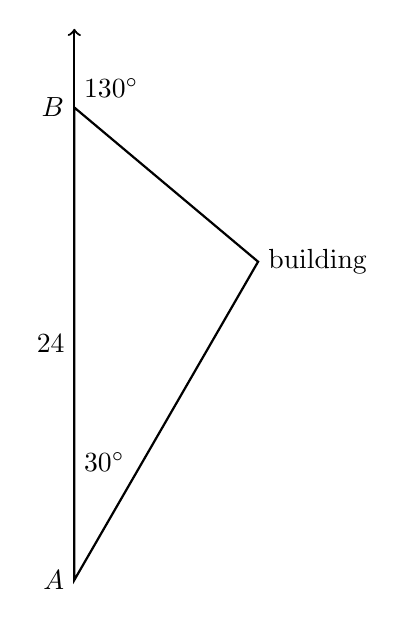
\begin{tikzpicture}[scale=0.25]
    \draw [thick]
    (-40:12.185)node[right]{building}--
    (0,0)node[left]{$B$}--
    (0,-24)node[left]{$A$}--cycle;
    \draw [thick, ->] (0,0)--(0,4);
    \node at (0,-12)[left]{$24$};
    \node at (0,-18)[right]{$30^\circ$};
    \node at (0,1)[right]{$130^\circ$};
  \end{tikzpicture}
\end{center}

\item A triangular field has boundaries of length 120 m, 145 m, and 155 m. 
\begin{enumerate}
  \item Find the size of the smallest interior angle of the field. \hfill (3 marks)
  \item Hence find the area of the field. \hfill (3 marks)
\end{enumerate}

\newpage
\item The following diagram shows quadrilateral $ABCD$ (not drawn to scale).
  \begin{center}
    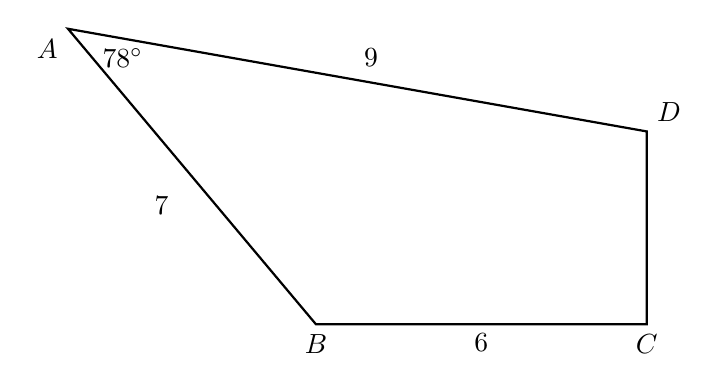
\begin{tikzpicture}[scale=0.7]
      \draw [-, thick] (130:7) node[below left]{$A$}--
        (0,0) node[below]{$B$}--
        (6,0) node[below]{$C$}--
        (6,3.5) node[above right]{$D$} -- cycle;            
      \node at (130:6.3)[right]{$78^\circ$};
      \node at (1,4.5)[above]{$9$};
      \node at (3,0)[below]{$6$};
      %\node at (78:3.5)[below]{$4.2$};
      \node at (-2.8,2.5)[below]{$7$};
    \end{tikzpicture}
    \end{center} 
    $AB=8.0$, $BC=5.1$, $CD=4.2$, $AD=8.3$, and $B\hat{C}D=78^\circ$
    \begin{enumerate}
      \item Find the perimeter of the quadrilateral. \hfill [5 marks]
      \item Find the area of the quadrilateral. \hfill [3 marks]
    \end{enumerate}

\item For parallel resistors in an electrical circuit, the total resistance $R_{TOT}$ is given by the formula 
$$ \frac{1}{R_{TOT}} = \frac{1}{R_1} + \frac{1}{R_2}$$
Given that the resistances of two resistors are $R_1 = 5.4 \Omega$ and $R_2 = 2.7 \Omega$, each measured to the nearest ohm.
\begin{enumerate}
  \item Find the upper and lower bounds of the total resistance. \hfill (6 marks)
  \item Given that the actual resistance of the circuit is 1.8 ohms, find the range of percentage errors that could be obtained for $R_{TOT}$. \hfill (4 marks)
\end{enumerate}

\item A triangle field is shown with two sides measuring 70 m and 250 m. The measured sides meet at $65^\circ$ at point $A$. A horse is tied to a stake at point $A$ with a 70 m line so that it can graze within the sector marked. \\[0.25cm]
Find the area of the field that the horse cannot reach. \hfill (6 marks)
  \begin{center}
    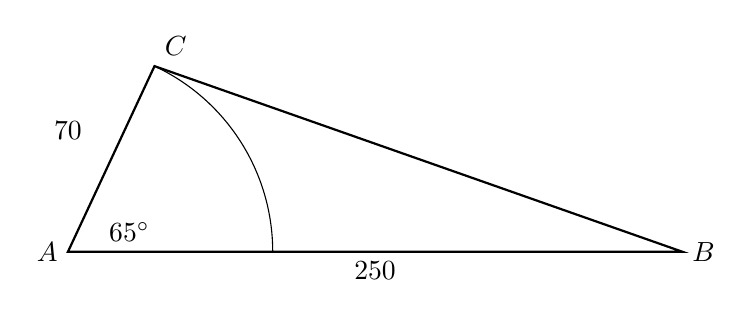
\begin{tikzpicture}[scale=1.3]
      \draw [-, thick] (65:2) node[above right]{$C$}--
        (0,0) node[left]{$A$}--
        (6,0) node[right]{$B$}--cycle;
      \draw (2,0) arc (0:65:2);
      \node at (0.6, 0)[above]{$65^\circ$};
      \node at (0, 1)[above]{$70$};
      \node at (3, 0)[below]{$250$};
    \end{tikzpicture}
    \end{center}



\newpage
   \item In right triangle $ABC$, hypotenuse $\overline{AB}$ has a length of 26 cm, and side $\overline{BC}$ has a length of 17.6 cm. What is the measure of angle $B$?

\newpage
\subsubsection*{Triangle area sine formula}
   \item Find the area of triangle $ABC$, with $AB=15$, $AC=17$, $m\angle A = 52^\circ$. \\[0.5cm]
   Hint: To use the area formula $A = \frac{1}{2} bh$ first find the altitude using sine and the hypotenuse $AC=17$.
   \begin{flushleft}
     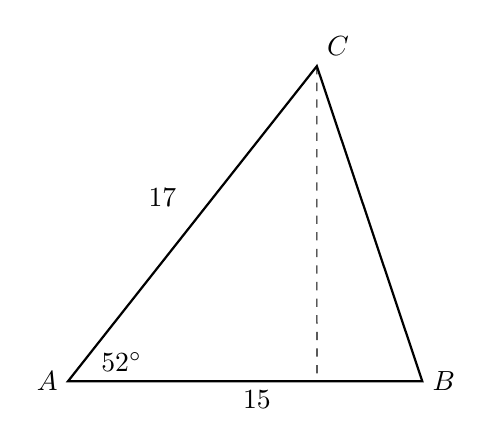
\begin{tikzpicture}[scale=0.3]
       \draw [-, thick] (51.7:17) node[above right]{$C$}--
         (0,0) node[left]{$A$}--
         (15,0) node[right]{$B$}--cycle;
       \node at (1, 0)[above right]{$52^\circ$};
       \node at (5, 7)[above left]{$17$};
       \node at (8, 0)[below]{$15$};

     \draw [-, dashed] (51.7:17)--(10.54,0);

     \end{tikzpicture}
     \end{flushleft} 

\newpage
\subsubsection*{Law of cosines}
  \item Solve the given triangle (determine the values of all lengths and angles)
  \begin{center}
    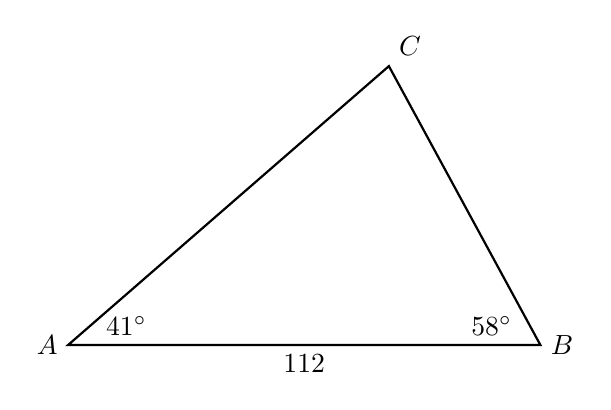
\begin{tikzpicture}[scale=1.2]
      \draw [-, thick] (41:4.5) node[above right]{$C$}--
        (0,0) node[left]{$A$}--
        (5,0) node[right]{$B$}--cycle;
      \node at (0.3, 0)[above right]{$41^\circ$};
      \node at (4.8, 0)[above left]{$58^\circ$};
      \node at (2.5, 0)[below]{$112$};
    \end{tikzpicture}
    \end{center}

\newpage
\subsubsection*{Law of sines}
  \item The following diagram shows triangle $ABC$ (not drawn to scale).
  \begin{center}
    \begin{tikzpicture}[scale=1.4, rotate=-25]
      \draw [-, thick] (50:3.5) node[above right]{$C$}--
        (0,0) node[left]{$A$}--
        (5,0) node[right]{$B$}--cycle;
      \node at (0.3, 0.15)[right]{$50^\circ$};
      \node at (4.5, 0.3)[above left]{$43^\circ$};
      \node at (3.7, 1.8)[below]{$11$};
    \end{tikzpicture}
    \end{center} 
    $BC=11$, $C\hat{A}B=50^\circ$, and $A\hat{B}C=43^\circ$
    \begin{enumerate}
      \item Find $AC$. \hfill [3 marks]
      \item Find the area of triangle $ABC$. \hfill [3 marks]
    \end{enumerate}

\newpage
  \item The following diagram shows quadrilateral $ABCD$ (not drawn to scale).
  \begin{center}
    \begin{tikzpicture}[scale=1.5, rotate=-20]
      \draw [-, thick] (100:3.5) node[above right]{$D$}--
        (0,0) node[below]{$B$}--
        (-5,0) node[below]{$A$}--cycle;
      \draw [-, thick] (100:3.5) --
      (55:3) node[right]{$C$}--
      (0,0);             
      \node at (58:2.9)[left]{$78^\circ$};
      \node at (50:1.5)[right]{$5.1$};
      \node at (-2.5,-0.2)[below]{$8.0$};
      \node at (78:3.5)[below]{$4.2$};
      \node at (-3,2.2)[below]{$8.3$};
    \end{tikzpicture}
    \end{center} 
    $AB=8.0$, $BC=5.1$, $CD=4.2$, $AD=8.3$, and $B\hat{C}D=78^\circ$
    \begin{enumerate}
      \item Find $BD$. \hfill [3 marks]
      \item Find $A\hat{B}D$. \hfill [3 marks]
    \end{enumerate}

\newpage
\subsubsection*{Precision application}
  \item BMI is a measure of a healthy personal weight, 
  \[\displaystyle BMI = \frac{w}{h^2}\]
    where \\
    $w$ is a person's weight in kilograms, and \\
    $h$ is height in meters
    \begin{enumerate} 
        \item Given a height of 160 cm and weight of 54 kg, find the BMI  \hfill [3 marks]
        \item These measurements are not exact. Assuming the height is between 159-161 cm and weight 53-55 kg, find the bounds of the BMI.  \hfill [4 marks]
      \end{enumerate}

\newpage
\subsubsection*{Sine ambiguous case}
  \item Triangle $ABC$ has an area of 25, with $AB=7$ and $AC=8$. 
  \begin{enumerate}
    \item Find the two possible measures for $\hat{A}$. \hfill [4 marks]
    \item Given that $\hat{A}$ is obtuse, find $BC$. \hfill [3 marks]
  \end{enumerate}

\newpage
\subsubsection*{Solid geometry}
\item Find the slant height of a pyramid with square base 4 meters on a side and height of 4 m. \hfill [3 marks]


  \item Find the volume of a spherical balloon 36 meters in diameter. \hfill [3 marks]
  
  \item A cone has a height of 24 cm and volume of $220.5\pi \,\mathrm{ cm}^3$. Find its radius. \hfill [3 marks]
  


\end{enumerate}
\end{document}
